\section{Stellar Structure \& Evolution} %
\label{sec:evolution}
\begin{shaded}
\noindent In this section, I will provide a summary of background information on the theory of stellar structure and evolution, with a focus toward the creation of evolutionary models of solar-like stars. 
This will allow us to state the evolution inverse problem: i.e., given observations of a star, to determine its age and evolutionary history. 
Stellar evolution is a well-established field with a rich history and many seminal works on the topic.  Textbooks overviewing the underpinnings of stellar structure and evolution are numerous and include works by \cite{1926ics..book.....E}, \cite{1939isss.book.....C}, \cite{1958ses..book.....S}, \cite{1989fsa..book.....C}, \cite{1990sse..book.....K}, \cite{1994sipp.book.....H}, \cite{2005essp.book.....S}, \cite{pols}, \cite{2012sse..book.....K}, and \cite{brown}. 
The following makes heavy use of these works, along with calculations using the stellar evolution code \emph{Modules for Experiments in Stellar Astrophysics} \citep[\textsc{MESA},][%
]{2011apjs..192....3p, 2013apjs..208....4p, 2015apjs..220...15p, 2018ApJS..234...34P}. \end{shaded}

Positing that a star begins as an initially homogeneous cloud of mostly hydrogen that collapses under its own weight until the conditions are ripe for fusion to sustain it, stellar evolution is the collection of physical processes that cause the star to vary over time from this state. 
Reposition in terms of luminosity, radius, density, and color---diagnostics that are visible from the stellar surface---are then predicted from the ensemble of processes that cause the star to transform. 

Many such processes are known. 
Nuclear fusion causes adjustment to the elemental abundances in the core or within shells inside the star. 
Gravitational settling causes heavier elements to sink inward, and radiative levitation selectively resists this sinking. 
Convection induces chemical mixing, which leads to chemical discontinuities when the boundaries of convective zones recede, and dredge-up events when an enveloping convective zone deepens into an area of disparate composition. 
Stars rotate, and this similarly causes material to mix. 
Magnetic fields, binary accretion, thermohaline mixing, and other processes may affect the evolution of stars as well. 


This collection of processes---of which only a subset is ``canonically'' employed in stellar modelling---has been very successful at explaining both the occupations of stars in the Hertzsprung-Russell and Color-Magnitude diagrams, and in predicting the pulsations of stars as well. 
Asteroseismic theory, visited in detail in the section following this one, is capable of determining the character of the stellar oscillations during each stage in a star's life, as well as predicting their corresponding periods. For solar-type stars, these predictions are within seconds of their measured values. 


\subsubsection*{Assumptions}
The standard theory describing the evolution of a single star follows from a number of basic assumptions:
\begin{enumerate}%
    \item \emph{Stars can be treated as a fluid.} 
    I make this assumption so that we may describe stars using the equations of fluid dynamics rather than considering the motions of individual particles. 
    The fluid approximation is likely a good description for the majority of the stellar interior, but it breaks down above the stellar photosphere. 
    \item \emph{Stars are isolated in space.} 
    I ignore companions and, consequently, the effects of mass transfer and tidal interactions. 
    \item \emph{Stars are spherically symmetric.} 
    I will describe the structure of a star from its core to its surface using only one coordinate (e.g.~radius, but in practice, some quantity that varies monotonically with radius). 
    I ignore rotation, which would distort the star. 
    While all stars rotate, many (such as the Sun) rotate slowly enough that the effects of rotation on their structure can be considered negligible. 
    \lr{\item \emph{Stars are self-gravitating.} 
    I include the effects of a gravitational field, but I ignore electric and magnetic fields. %
    \item \emph{Stars are dynamically stable.} 
    Clearly, stars are pulsating; that is the main subject of this thesis. 
    However, the pulsation timescale is usually much shorter than the evolutionary timescale. 
    These will be treated in detail in the next section. 
    \item \emph{Stars keep their mass.}
    Stars are observed to lose their mass through, for example, stellar winds. 
    However, isolated main-sequence stars lose very little mass. 
    For example, the Sun loses only about one part in $10^{13}$ of its mass each year \citep{2004CeMDA..90..267K}.}
\end{enumerate}
From these assumptions, we may now formulate equations for the structure of a star. 

\subsubsection*{Stellar Structure}
By the structure of a star, I mean the \emph{mechanical} (density $\rho$, pressure $P$), \emph{thermal} (temperature $T$, adiabatic exponents $\boldsymbol\Gamma$), and \emph{chemical} (relative abundances of hydrogen $X$, helium $Y$, and heavy elements $Z$ obeying ${X+Y+Z=1}$) profiles from the core to the `surface.' 
The equations of stellar structure consist of three conservation equations---conservation of mass, momentum, and energy---and the temperature equation. 
These macrophysical equations are supplemented with `microphysics,' numerical inputs for necessary ingredients such as nuclear reaction rates. 
I will present most of the equations of stellar structure essentially without derivation. 
In order to give the reader an idea of the arguments used, however, I will provide derivations based on geometry and basic physics for the conservation of mass and the conservation of (linear) momentum. 

It is natural to consider these quantities spatially (i.e., in one dimension, by the stellar radius). 
However, the radius of a star changes considerably over its lifetime, growing from a dwarf to a giant and then becoming a dwarf again. 
On the other hand, the mass of a star, at least in the main-sequence phase, is very stable. 
The Sun, for example, loses only $10^{-14}$ of its mass per year through fusion and the solar wind. 
Therefore, I will here cast the equations using mass as the independent variable. 
In practice, stellar evolution codes often use a more complex variable which is even more stable than mass. 

\begin{description}%
    \setlength{\itemindent}{0pt}
    \item[Conservation of Mass.]
    Geometrically speaking, the mass $m$ contained within a sphere spanning from the centerpoint (${r=0}$) to a radius of $r$ is given by 
    \lr{\begin{equation}
        m(r)
        =
        \int_0^r 4 \pi x^2 \rho(x) \; \text{d}x.
    \end{equation}}
    Differentiating this equation, and dropping arguments, we arrive at 
    \begin{equation} \label{eq:cons-mass} \boxed{
        \frac{\text{d}r}{\text{d}m}
        =
        \frac{1}{4\pi r^2\rho}
    }\end{equation}
    which, as we will see, is the continuity equation in the absence of flows. $\hfill\square\;$
    
    \item[Conservation of Momentum.] 
    The state of balance between gravity and a pressure-gradient force is called hydrostatic support (also known as hydrostatic equilibrium or hydrostatic balance) and is a special case of conservation of momentum. 
    The equation can be derived from either Newton's laws of motion, the Navier--Stokes equations, or from general relativity. 
    Here I show the former. 
    
    Consider a small fluid parcel inside of the star whose base is located at radius $r$ having height ${\text{d}r}$ and a constant area $A$. 
    The parcel has three forces acting upon it: downward and upward forces from pressure, and a downward force from gravity. 
    The upward force on the parcel is 
    \begin{equation}
        F_{\text{upward}} (r) = A \cdot \underbrace{P(r)}_{\makebox[0pt]{\text{\scriptsize pressure below}}}
    \end{equation}
    and the combined downward force is
    \begin{equation}
        F_{\text{downward}} (r)
        = -\left(
            A \cdot \underbrace{P(r+\text{d}r)}_{\makebox[0pt]{\text{\scriptsize pressure above}}} + \underbrace{A \cdot \rho(r) g(r) \cdot \text{d}r}_{\text{gravity}}
        \right).
    \end{equation}
    When these forces are balanced, i.e.~${F_{\text{upward}} = F_{\text{downward}}}$, the parcel is said to be in hydrostatic equilibrium. 
    Thus, we have
    \begin{equation}
        0 = 
        -A\left( 
                \mathrlap{\underbrace{\phantom{\;P(r)}}_{F_{\text{upward}}}}
                \;\mathrlap{\overbrace{\phantom{P(r) - P(r+\text{d}r)}}^{\text{d}P}}
                P(r) - 
                \underbrace{
                    P(r+\text{d}r) - \rho(r) g(r) \cdot \text{d}r
                }_{F_{\text{downward}}}
        \right)
    \end{equation}
    which then gives us
    \begin{align} \label{eq:cons-mom-r}
        \frac{\text{d} P}{\text{d} r} &= -\rho g.
    \end{align}
    We may then apply the equation of conservation of mass (\ref{eq:cons-mass}) and obtain
    \begin{equation} \label{eq:cons-mom} \boxed{
        \frac{\text{d} P}{\text{d} m} = -\frac{Gm}{4\pi r^4}
    }\end{equation}
    where ${G = 6.67408\times 10^{-8}}$~\si{\per\g\cm\cubed\per\square\s} is the gravitational constant. $\hfill\square\;$
    
    These two conservation equations give us the mechanical structure of the star---the pressure and density throughout the stellar interior. 
    Assuming a constant temperature, the ratio of these quantities gives us the speed at which acoustic waves propagate in the star:
    \begin{equation} \label{eq:u}
        u = P/\rho.
    \end{equation}
    This quantity is known as the \emph{\lr{squared} isothermal speed of sound} and will be important in the following investigations. 
    
    \item[Conservation of Energy.]
    The flow of energy $l$ throughout the stellar interior is given by 
    \begin{equation} \label{eq:energy} \boxed{
        \frac{\text{d}l}{\text{d}m}
        =
        \epsilon_{\text{nuc}} - \epsilon_\nu + \epsilon_g %
    }\end{equation}
    where $\epsilon_{\text{nuc}}$ is the energy generated by nuclear reactions, $\epsilon_\nu$ is the energy lost by neutrinos, and $\epsilon_g$ is the gravitational energy from expansion or compression: %
    \begin{equation} \label{eq:eps-g}
        \epsilon_{\text{g}} = -T\, \frac{\partial s}{\partial t}
    \end{equation}
    where $s$ is the specific entropy. 
    The nuclear energy generation rates are supplied externally. 
    Here I use the rates from the \emph{Nuclear Astrophysics Compilation of Reaction Rates} \citep[\textsc{NACRE},][]{1999NuPhA.656....3A}. 
    The neutrino energy loss rates can be calculated using the formulas given by \citet{1996ApJS..102..411I}. 
    
    
    Computing the $\epsilon_g$ term requires an equation of state (EOS). 
    This too is supplied externally. For the low-mass stars considered here, I use the \emph{Opacity Project at Livermore} EOS \citep[\textsc{OPAL},][]{2002apj...576.1064r}. 
    The EOS relates the pressure, density, and temperature of the stellar matter to each other in a thermodynamically-consistent manner. 
    The adiabatic exponents $\boldsymbol\Gamma$, introduced by Chandrasekhar, give these relations as follows: %
    \begin{align} 
        \Gamma_1 
        &= 
        \left(
            \frac{\partial \ln P}{\partial \ln \rho}
        \right)_{\text{ad}} 
        \\
        \frac{\Gamma_2}{\Gamma_2-1}
        &= \label{eq:gamma2}
        \left(
            \frac{\partial \ln P}{\partial \ln T}
        \right)_{\text{ad}} = \frac{1}{\nabla_{\text{ad}}}
        \\
        \Gamma_3 - 1 
        &= 
        \left(
            \frac{\partial \ln T}{\partial \ln \rho}
        \right)_{\text{ad}}
    \end{align}
    which are related to each other as: 
    \begin{equation}
        \frac{\Gamma_1}{\Gamma_3 - 1}
        =
        \frac{\Gamma_2}{\Gamma_2-1}.
    \end{equation}
    The first adiabatic exponent describes how the compression of a layer changes the pressure in that layer, which, as we will see, is important for determining dynamical stability, i.e., stellar pulsations. 
    In particular, \lr{in an anisotropic ideal gas,} the speed at which acoustic waves propagate---the adiabatic speed of sound\footnote{ Not to be confused with the speed of light.}---can be defined as 
    \begin{equation} \label{eq:speed-of-sound}
        c = \sqrt{\Gamma_1 u}. 
    \end{equation}
    The second adiabatic exponent describes how changes in pressure impact upon the temperature, which is important for determining stability against convection. 
    In an ideal monoatomic gas, the adiabatic exponents all equal $5/3$. %

    
    
    \item[Temperature Equation.]
    The temperature throughout the star is given by 
    \begin{equation} \label{eq:temperature} \boxed{
        \frac{\text{d}T}{\text{d}m}
        =
        -\frac{Gm}{4\pi r^4} \frac{T}{P} \nabla_T
    }\end{equation}
    where $\nabla_T$ is a dimensionless temperature gradient:
    \begin{equation}
        \nabla_T 
        =
        \frac{\text{d}\ln T}{\text{d}\ln P}
    \end{equation}
    whose form depends on the mode of energy transport. 
    In the case of pure radiation,
    \begin{equation} \label{eq:radiative-gradiant}
        \nabla_T 
        = 
        \nabla_{\text{rad}} 
        =
        \frac{3}{64\pi \sigma G}
        \frac{\kappa l P}{m T^4}.
    \end{equation}
    where \lr{${\sigma = 5.670367 \cdot 10^{-5} \; \text{erg}\; \text{cm}^{-2}\; \text{s}^{-1}\; \text{K}^{-4}}$}
    is the Stefan-Boltzmann constant and $\kappa$ is the opacity of the stellar matter, which is also supplied externally. 
    Here I use the \textsc{OPAL} opacities \citep{1996ApJ...464..943I}. 
    
    The conductive temperature gradient is negligible for our purposes, though it is relevant e.g.~in white dwarfs. 
    The convective temperature gradient comes from both the adiabatic gradient of the assumed EOS (\emph{cf.}~Equation~\ref{eq:gamma2}) and the specific treatment of convection, which I will discuss later in this section. 
    \iffalse
    In the case of convection, and ignoring superadiabaticity, 
    \begin{equation}
        \nabla_T
        =
        \nabla_{\text{ad}} 
        =
        \left(
            \frac{\partial \ln T}{\partial \ln P}
        \right)_{\text{ad}}
    \end{equation}
    where an adiabatic derivative is taken at constant specific entropy, which comes from the EOS. 
    \fi
\end{description}

\noindent We thus have four coupled differential equations (\ref{eq:cons-mass}, \ref{eq:cons-mom}, \ref{eq:energy}, \ref{eq:temperature}) that govern stellar structure. 
In order to solve them, we will need four boundary conditions. 

\subsubsection*{Boundary Conditions}

The first boundary is at the central point in the star, where ${m=0}$.
Here we have %
\begin{equation}
    m=0,\qquad r=0,\qquad l=0.
\end{equation} 
The second boundary is at the stellar surface. %
This is where the mass equals the total mass, ${m=M}$; and where the radius equals the total radius, ${r=R}$. 
A simple option is to assume that the temperature and pressure vanish at the surface, i.e.
\begin{equation} \label{eq:zero}
    T(r=R)=0, \qquad P(r=R)=0.
\end{equation}
These are known as \emph{zero-boundary} conditions and we will make use of them later when calculating variational pulsation mode frequencies (see Section~\ref{sec:variational}). 
They are unrealistic, however, as even the interstellar medium has a non-zero temperature. 

A more sophisticated option is to call the surface the region where majority of the radiation escapes from the star, i.e., the photosphere. 
Here I will use a standard Eddington gray atmosphere, which gives the total luminosity and effective temperature 
\begin{equation}
    l(r=R) = L,\qquad T(r=R) = T_{\text{eff}}
\end{equation}
following the Stefan-Boltzmann Law %
for blackbody radiation: 
\begin{align} \label{eq:stefan-boltzmann} 
    L &= 4\pi R^2 \sigma T_{\text{eff}}^4
\end{align}
where $\sigma$ is again the Stefan-Boltzmann constant. %
Finally, the pressure at the surface is given by 
\begin{equation}
    P(r=R)
    =
    \frac{2}{3} 
    \frac{GM}{R^2}
    \frac{1}{\bar \kappa}
\end{equation}
where $\bar \kappa$ is the Rosseland mean opacity. 




\subsubsection*{Stellar Evolution}
For a star to \emph{evolve}, it must change over time. With the exception of one term for the gravitational energy from expansion or compression (Equation~\ref{eq:eps-g}), the equations of stellar structure feature no time derivatives; %
they describe a static star. 
The equations of stellar structure may be supplemented with time-dependent evolution equations describing the internal transport or modification of chemical species. 

\begin{description}
    \setlength{\itemindent}{0pt}
    \item[Nuclear reactions.] Energy generation on the main sequence stems predominately from the conversion of hydrogen atoms (H) into helium atoms (He). 
    The net reaction is 
    \begin{equation}
        4\;^1\text{H}\; \rightarrow\; ^4\text{He} + 2\text{e}^+ + 2\nu_{\text{e}}
    \end{equation}
    where e$^+$ is a positron and $\nu_{\text{e}}$ is a neutrino. 
    Earth-based detections of neutrinos matching the predicted solar output essentially confirm this description. 
    The evolution due to nuclear reactions can be given as: 
    \begin{equation} \boxed{
        \frac{\partial X_i}{\partial t}
        =
        \frac{m_i}{\rho}
        \left( 
            \sum_j r_{ji}
            -
            \sum_k r_{ik}
        \right)
    }\end{equation}
    where $X_i$ is the $i^{\text{th}}$ isotope, $m_i$ is the mass of that isotope, and $r_{i,j}$ is the rate at which $X_i$ is formed from $X_j$. 
    As mentioned, these rates must be supplied externally; here I've chosen to use the \textsc{NACRE} rates. 
    
    \item[Diffusion.] The processes of element diffusion and the gravitational settling of helium and heavy elements can be included via \lr{the diffusion equation: 
    \begin{equation} \label{eq:evol-diffusion} \boxed{
        \frac{\partial X_i}{\partial t}
        =
        D_i\, \frac{\partial^2 X_i}{\partial m^2}
    }\end{equation}
    where $D_i$ is the diffusion coefficient for isotope $X_i$.} 
    Diffusion coefficients must also be externally supplied; a common choice are those of \citealt{1994ApJ...421..828T}.
    
    \item[Convection.] 
    According to the Schwarzschild criterion \citep[e.g.,][]{1958ses..book.....S}, a region is unstable to convection when the radiative gradient exceeds the adiabatic gradient: 
    \begin{equation}
        \nabla_{\text{rad}} 
        > 
        \nabla_{\text{ad}}
    \end{equation}
    (\emph{cf.}~Equations~\ref{eq:gamma2} and~\ref{eq:radiative-gradiant}). 
    Here I will treat convection using the standard \citet{1958ZA.....46..108B} mixing length theory, which approximates the effects of convection by assuming that convective elements travel to some characteristic length $\ell_m$ before mixing the transported material with their newfound surroundings. %
    The mixing length is controlled by a free parameter $\alpha_{\text{MLT}}$, which is scaled by the local \lr{pressure scale height: 
    \begin{align} \label{equation:MLT}
        \ell_m
        &=
        \alpha_{\text{MLT}} \cdot H_p\\
        H_p
        &=
        -\left(\frac{\text{d} \ln P}{\text{d}r}\right)^{-1}.
    \end{align}}
    There is no \emph{a priori} choice for $\alpha_{\text{MLT}}$. 
    Generally, $\alpha_{\text{MLT}}$ is either fixed to a value that has been calibrated to the observed characteristics of the Sun, which we shall address later in this section; or fit on a star-by-star basis (Chapter~\ref{chap:ML}). 
    
    Convection is an efficient mixer. %
    We can model the changes to chemical abundances due to convection as a diffusion process:
    \lr{\begin{equation} \boxed{
        \frac{\partial X_i}{\partial t}
        =
        \frac{\partial}{\partial m} \left( 
            D_{\text{conv}}\, \frac{\partial X_i}{\partial m}
        \right)
    }\end{equation}}
    where ${D_{\text{conv}} \propto v_c \cdot \ell_m}$, with $v_c$ being the convective velocity.
    
    Convective zones can be extended beyond their normal boundaries via convective overshooting. 
    Overshooting is similarly controlled by a free parameter $\alpha_{\text{ov}}$, which extends the boundary by ${\alpha_{\text{ov}} \cdot H_p}$. 
    Like $\alpha_{\text{MLT}}$, the overshooting parameter has no predefined value. 
    While it is not uncommon to exclude the effects of overshooting altogether, $\alpha_{\text{ov}}$ can also be determined from a fit to a stellar population \citep[e.g.,][]{2005ARA&A..43..387G} or on a star-by-star basis (Chapter~\ref{chap:ML}). 
\end{description}

\noindent Calculations generally proceed as follows. 
First, the equations of stellar structure are solved for a given composition. 
Then, time is advanced, and a new composition is computed using the evolution equations. 
The equations of stellar structure are then solved again for the new composition, and the procedure is repeated. 
\citet{1959ApJ...129..628H} introduced an efficient scheme to solve these equations based on iterative application of the Newton-Raphson method. 
We will now solve these equations and model the evolution of the stars. %


\subsubsection*{Solar Calibration}
\label{sec:calibration}

We may begin our calculations by calibrating an evolutionary track to the observed properties of the Sun \citep[e.g.][]{1982MNRAS.199..735C} in accordance with the recommended nominal solar values adopted by the IAU \citep{2015arXiv151007674M}. 
The standard gravitational parameter of the Sun $\mu_\odot$ is known to very high precision from planetary orbits: 
\begin{equation*}
    \mu_\odot = GM_\odot = 1.3271244 \cdot 10^{26} \; \text{cm}^3 \; \text{s}^{-2}.
\end{equation*}
The gravitational constant may be determined experimentally; this then yields the solar mass. 
Next, the Earth-Sun distance as well as direct observations give the solar radius. 
Solar irradiance measurements give the solar luminosity. 
Spectroscopy gives the composition the solar photosphere; I use the mixture as measured by \citet[][hereinafter \textsc{GS98}]{1998SSRv...85..161G} which gives good agreement with helioseismology. 
Finally, radiometric dating of meteorites gives the age of the solar system. 
Putting this all together, the Sun has the following characteristics: 
\lr{\begin{equation} \label{eq:solar-vals}
\begin{aligned}
    \text{mass } M_\odot &= 1.988475 \cdot 10^{33}\; \text{g} \\
    \text{radius } R_\odot &= 6.957 \cdot 10^{10}\; \text{cm} \\
    \text{luminosity } L_\odot &= 3.828 \cdot 10^{33}\; \text{erg}\; \text{s}^{-1} \\
    \makebox[0pt][r]{\text{effective }}\text{temperature } T_{\text{eff},\odot} &= 5772\; \text{K} \\
    \makebox[0pt][r]{\text{heavy mass fraction }} (Z/X)_\odot &= 0.02293 \\
    \text{age } \tau_\odot &= 4.572\cdot 10^{9} \; \text{yr}.
\end{aligned}
\end{equation}}
These are the values that must be reproduced in our solar calibration. 
We will achieve this by altering the initial chemical composition and the efficiency of convective mixing (recall Equation~\ref{equation:MLT}) until these values are reproduced at the solar age. 
Since the Sun is an isolated main-sequence star, its mass has been presumably very stable throughout its lifetime. 
The initial mass of the calibration can therefore remain fixed at the solar value. 
Finally, we only need to check that e.g.~the luminosity and radius are matched, since $R, L,$ and $T_{\text{eff}}$ are related through the Stefan-Boltzmann Law (Equation~\ref{eq:stefan-boltzmann}).

We therefore have the following optimization problem: 
we wish to tune the initial helium abundance $Y_0$, initial metallicity $Z_0$, and mixing length parameter $\alpha_{\text{MLT}}$ of a solar-mass track such that we minimize ${\log\left(L/L_\odot\right)}$,  ${\log\left(R/R_\odot\right)}$, and [Fe/H] at the solar age, where [Fe/H] is defined as
\begin{equation}
    \text{[Fe/H]}
    \equiv
    \log\left( \frac{Z}{X} \right)_\ast
    -
    \log\left( \frac{Z}{X} \right)_\odot.
\end{equation}
We may achieve solar calibration by, e.g., iterative application of Newton's rule: 
\begin{equation}
    \mathbf{x}_{t+1}
    =
    \mathbf{x}_t - \mathbf{J}_t^{-1} \mathbf{f}(\mathbf{x}_t)
\end{equation}
where (dropping the $\text{MLT}$ and $0$ subscripts)
\begin{align}
    \mathbf{x}_t
    &=
    \begin{pmatrix} Y_t , & Z_t , & \alpha_t \end{pmatrix}
    \\
    \mathbf{f}(\mathbf{x}_t)
    &=
    \begin{pmatrix} 
        \log \left\{ L_t/L_\odot \right\}, &
        \log \left\{ R_t/R_\odot \right\}, &
        \text{[Fe/H]}_t
    \end{pmatrix}
\end{align}
\begin{equation}
    \mathbf{J}_t
    =
    \begin{pmatrix} 
        \dfrac{\strut\partial \log \left\{ L_t/L_\odot \right\}}{\strut\partial Y} &
        \dfrac{\strut\partial \log \left\{ L_t/L_\odot \right\}}{\strut\partial Z} &
        \dfrac{\strut\partial \log \left\{ L_t/L_\odot \right\}}{\strut\partial \alpha}\\
        \dfrac{\strut\partial \log \left\{ R_t/R_\odot \right\}}{\strut\partial Y} &
        \dfrac{\strut\partial \log \left\{ R_t/R_\odot \right\}}{\strut\partial Z} &
        \dfrac{\strut\partial \log \left\{ L_t/L_\odot \right\}}{\strut\partial \alpha}\\
        \dfrac{\strut\partial \text{[Fe/H]}_t}{\strut\partial Y} &
        \dfrac{\strut\partial \text{[Fe/H]}_t}{\strut\partial Z} &
        \dfrac{\strut\partial \text{[Fe/H]}_t}{\strut\partial \alpha}
    \end{pmatrix}.
\end{equation}
Here $t$ refers to the $t^{\text{th}}$ iteration, and the partial derivatives are to be calculated numerically (i.e.\ by running tracks with small changes to those parameters). 
It may also be prudent to enforce some box constraints, for example: ${0.23 \leq Y_0 \leq 0.33}$, ${0 < Z_0 < 0.05}$, ${1 \leq \alpha_{\text{MLT}} \leq 3}$. 
When supplied with a reasonable initial guess, this scheme eventually converges onto a set of parameters that reproduce the observed solar values: 
\begin{alignat}{3} \label{eq:solar-cal-vals} 
    &Y_0 &&\simeq 0.273  &\log(L/L_\odot) &\simeq 0 \notag\\
    &Z_0 &&\simeq 0.019 \qquad\Rightarrow\qquad &\log(R/R_\odot) &\simeq 0\\\notag
    &\alpha_{\text{MLT}} &&\simeq 1.84  &\text{[Fe/H]} &\simeq 0.
\end{alignat}
These initial values, as well as the observed values of the Sun (Equations~\ref{eq:solar-vals}) are the ones that will need to be reproduced when we later perform evolutionary inversions on degraded Sun-as-a-star data (see Chapter \ref{chap:ML}), where they are all either unknown or highly uncertain. 

We may now inspect the structure of our solar model. 
Figure~\ref{fig:profs} shows some aspects of the mechanical, thermal, and chemical structure of the model. 
Helioseismology has revealed that these profiles are exceptionally close to the actual interior of the Sun \citep[see, e.g.,][]{2016lrsp...13....2b}. 

A few points are worthy of note here. 
The first adiabatic exponent is close to ${5/3}$ (i.e., nearly the conditions of an ideal gas) for the majority of the solar interior and only deviates from this value close to the solar surface. 
The helium abundance $Y$ in the solar core is maximal due to nearly $5$~Gyr of hydrogen-to-helium fusion. 
Helium is now the dominant element in the core, with the fractional hydrogen abundance being reduced to $0.344$. 
Throughout the convection zone, which extends from ${\sim 0.7\;{r/R}}$ to the solar surface, the helium abundance has a constant value of $0.279$ due to convective mixing. 
This value is somewhat higher than the protosolar value of $0.273$ due to element diffusion. 

The density ranges from around $150$~g/cm$^3$ in the core to less than that of water in the outer half of the star, with the mean density of the Sun being about a hundredth of the core density. 
The pressure in the solar core falls off more rapidly than the density, which causes the speed of sound to rise temporarily when moving away from the centerpoint. 
Furthermore, since $u\propto T/\mu$, where $T$ is the temperature and $\mu$ is the mean molecular weight, the speed of sound in the solar core is related to the age of the Sun via the increased abundance of helium. 

\begin{figure}
    \centering
    \begin{subfigure}[b]{0.5\linewidth}
        \centering
        \includegraphics[width=\textwidth,keepaspectratio]{figs/pulse/diffs/prof_D-u.pdf}
    \end{subfigure}%
    \begin{subfigure}[b]{0.5\linewidth}
        \centering
        \includegraphics[width=\textwidth,keepaspectratio]{figs/pulse/diffs/prof_D-rho.pdf}%
    \end{subfigure}\\
    \begin{subfigure}[b]{0.5\linewidth}
        \centering
        \includegraphics[width=\textwidth,keepaspectratio]{figs/pulse/diffs/prof_D-Gamma1.pdf}%
    \end{subfigure}%
    \begin{subfigure}[b]{0.5\linewidth}
        \centering
        \includegraphics[width=\textwidth,keepaspectratio]{figs/pulse/diffs/prof_D-Y.pdf}%
    \end{subfigure}
    \caption[The Sun's internal mechanical, thermal, and chemical profile]{\lr{Squared isothermal sound speed} (top left), density (top right), first adiabatic exponent (bottom left), and fractional helium abundance (bottom right) profiles for a solar model. 
    \label{fig:profs} } 
    \vspace*{1cm}
    \includegraphics[width=\textwidth]{figs/evol/hr-solar.pdf}
    \caption[Solar H-R Diagram]{Hertzsprung-Russell diagram showing the evolution of the Sun. 
    The background colors correspond to spectral type (F, G, K, M). 
    The position of the Sun is indicated with the solar symbol ($\odot$). 
    \label{fig:solar-HR}}
\end{figure}


We may additionally inspect the resulting evolutionary path of the solar-calibrated track. 
Figure~\ref{fig:solar-HR} shows the past and future evolution of our Sun, assuming that the theory of stellar evolution is approximately correct; and Figure~\ref{fig:chem_ev} shows the chemical evolution of the solar core. 
The Sun is currently on the main sequence; after several billion years, it will cross the sub-giant branch, climb the red giant branch (RGB), reach the tip of the RGB, and then fall onto the red clump (RC). 
The configurations of the star at these points in its evolution are shown in Figure~\ref{fig:config}. 

\begin{figure}
    \centering
    \includegraphics[width=\textwidth]{figs/evol/chem_ev_sun_core.pdf}
    \caption[Chemical evolution of the solar core]{The past and future chemical evolution of the core of our Sun. The left panel shows the main sequence evolution, from the zero-age main sequence (ZAMS) to the terminal-age main sequence (TAMS). The right panel shows the evolution from the red giant luminosity bump through to the tip of the red giant branch and eventually to core-helium exhaustion. 
    The core composition does not change throughout the majority of the subgiant and red giant phases. 
    \label{fig:chem_ev}} 
    \vspace*{0.1cm}
\begin{minipage}[t][1cm][t]{1cm+\widthof{convection}}\vspace{0pt}
\begin{tikzpicture}[scale=3]
  \filldraw[fill=black!5!white]
    (0,0) -- (0.169,0) -- (.169,.1) -- (0,.1) -- (0,0);
  \filldraw[pattern=crosshatch dots, pattern color=black]
    (0,0) -- (0.169,0) -- (.169,.1) -- (0,.1) -- (0,0);
  \node[right] at (0.169, 0.06) {convection}; 
\end{tikzpicture}%
\end{minipage}
\begin{minipage}[t][1cm][t]{1cm+\widthof{radiation}}\vspace{0pt}
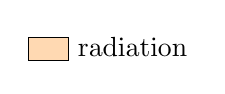
\begin{tikzpicture}[scale=3]
  \filldraw[fill=orange!30!white]
    (0,0) -- (0.169,0) -- (.169,.1) -- (0,.1) -- (0,0);
  \node[right] at (0.169, 0.06) {radiation}; 
\end{tikzpicture}%
\end{minipage}
\begin{minipage}[t][1cm][t]{1cm+\widthof{hydrogen fusion}}\vspace{0pt}
\begin{tikzpicture}[scale=3]
  \filldraw[pattern=fivepointed stars2, pattern color=red!70!black]
    (0,-0.04) -- (0.169,-0.04) -- (.169,.06) -- (0,.06) -- (0,-0.04);
  \node[right] at (0.169, 0) {hydrogen fusion}; 
\end{tikzpicture}%
\end{minipage}
\begin{minipage}[t][1cm][t]{1cm+\widthof{helium fusion}}\vspace{0pt}
\begin{tikzpicture}[scale=3]
  \filldraw[pattern=fivepointed stars3, pattern color=blue!70!black]
    (0,0) -- (0.169,0) -- (.169,.1) -- (0,.1) -- (0,0);
  \node[right] at (0.169, 0.06) {helium fusion}; 
\end{tikzpicture}
\end{minipage}

\vspace*{0.25cm}

\begin{tikzpicture}[scale=3] %
  \def\core{{(log10(0.2)-log10(0.001))/3}}
  \def\env{{(log10(0.7)-log10(0.001))/3}}
  \filldraw[fill=orange!30!white]
    (0,0) -- (1,0) arc (0:90:1) -- (0,0);
  \filldraw[fill=orange!15!white]%
    (0,0) -- (\core,0) arc (0:90:\core) -- (0,0);
  \filldraw[pattern=fivepointed stars2, pattern color=red!70!black]
    (0,0) -- (\core,0) arc (0:90:\core) -- (0,0);
  \filldraw[fill=black!5!white, draw=black]
    (\env, 0) -- (1, 0) arc (0:90:1) -- (0, \env) arc (90:0:\env);
  \filldraw[pattern=crosshatch dots, pattern color=black]
    (\env, 0) -- (1, 0) arc (0:90:1) -- (0, \env) arc (90:0:\env);
  \draw[color=black]
    (0,0) -- (1,0) arc (0:90:1) -- (0,0);
  \path[inner sep=0] (-0.03, 0) node[left] {$0.001$};
  \path[inner sep=0] (-0.03, {(log10(0.01)-log10(0.001))/3}) node[left] {$0.01$};
  \path[inner sep=0] (-0.03, {(log10(0.1)-log10(0.001))/3}) node[left] {$0.1$};
  \path[inner sep=0] (-0.03, {(log10(1)-log10(0.001))/3}) node[left] {$r/R = 1$};
  \path[inner sep=0] (0.94, 0.9) node {$0.9-1.3~R_\odot$}; 
  \path[inner sep=0] (0.5, -0.15) node {main sequence}; 
\end{tikzpicture}%
\hspace{0.5cm}
\begin{tikzpicture}[scale=3] %
  \def\shellbot{{(log10(0.01)-log10(0.001))/3}}
  \def\shelltop{{(log10(0.02)-log10(0.001))/3}}
  \def\env{{(log10(0.05)-log10(0.001))/3}}
  \filldraw[fill=orange!30!white]
    (0,0) -- (1,0) arc (0:90:1) -- (0,0);
  \filldraw[fill=orange!15!white]
    (\shellbot, 0) -- (\shelltop, 0) arc (0:90:\shelltop) -- (0, \shellbot) arc (90:0:\shellbot);
  \filldraw[pattern=fivepointed stars2, pattern color=red!70!black]
    (\shellbot, 0) -- (\shelltop, 0) arc (0:90:\shelltop) -- (0, \shellbot) arc (90:0:\shellbot);
  \filldraw[fill=black!5!white, draw=black]
    (\env, 0) -- (1, 0) arc (0:90:1) -- (0, \env) arc (90:0:\env);
  \filldraw[pattern=crosshatch dots, pattern color=black]
    (\env, 0) -- (1, 0) arc (0:90:1) -- (0, \env) arc (90:0:\env);
  \draw[color=black]
    (0,0) -- (1,0) arc (0:90:1) -- (0,0);
  \path[inner sep=0] (0.94, 0.9) node {$1.3-175~R_\odot$}; 
  \path[inner sep=0] (0.5, -0.15) node {sub/red giant}; 
\end{tikzpicture} %
\hspace{0.5cm}
\begin{tikzpicture}[scale=3] %
  \def\core{{(log10(0.002)-log10(0.001))/3}}
  \def\shellbot{{(log10(0.0063)-log10(0.001))/3}}
  \def\shelltop{{(log10(0.01)-log10(0.001))/3}}
  \def\env{{(log10(0.2213)-log10(0.001))/3}}
  \def\convcore{{(log10(0.0031)-log10(0.001))/3}}
  \filldraw[fill=orange!30!white]
    (0,0) -- (1,0) arc (0:90:1) -- (0,0);
  \filldraw[fill=black!5!white, draw=black]
    (0,0) -- (\convcore,0) arc (0:90:\convcore) -- (0,0);
  \filldraw[pattern=crosshatch dots, pattern color=black]
    (0,0) -- (\convcore,0) arc (0:90:\convcore) -- (0,0);
  \filldraw[pattern=fivepointed stars3, pattern color=blue!70!black]
    (0,0) -- (\core,0) arc (0:90:\core) -- (0,0);
  \filldraw[fill=orange!15!white]
    (\shellbot, 0) -- (\shelltop, 0) arc (0:90:\shelltop) -- (0, \shellbot) arc (90:0:\shellbot);
  \filldraw[pattern=fivepointed stars2, pattern color=red!70!black]
    (\shellbot, 0) -- (\shelltop, 0) arc (0:90:\shelltop) -- (0, \shellbot) arc (90:0:\shellbot);
  \filldraw[fill=black!5!white, draw=black]
    (\env, 0) -- (1, 0) arc (0:90:1) -- (0, \env) arc (90:0:\env);
  \filldraw[pattern=crosshatch dots, pattern color=black]
    (\env, 0) -- (1, 0) arc (0:90:1) -- (0, \env) arc (90:0:\env);
  \draw[color=black]
    (0,0) -- (1,0) arc (0:90:1) -- (0,0);
  \path[inner sep=0] (0.94, 0.9) node {$10-12~R_\odot$}; 
  \path[inner sep=0] (0.5, -0.15) node {red clump}; 
\end{tikzpicture}      \caption[Configurations of the solar interior]{The configuration of the solar interior as the Sun evolves. 
    The present Sun is a main-sequence star with a radiative core where hydrogen fusion is synthesizing helium. 
    The outer ${\sim 30\%}$ of the Sun by radius transports energy by convection. 
    When the Sun depletes its supply of core hydrogen in ${\sim 5}$~Gyr, it will continue burning hydrogen in a shell outside of the core. 
    For the next ${\sim 2.5}$~Gyr, the inert helium core will contract while the convective envelope deepens as the Sun puffs up into a giant star. 
    The Sun will then reach the tip of the red giant branch, where helium in the highly degenerate core will suddenly undergo a flash ignition. 
    The Sun will subsequently become a red clump star, where it will continue fusing hydrogen in a radiative shell while simultaneously fusing helium in its convective core. 
    \label{fig:config}}
\end{figure}

Subsequent to these stages is the asymptotic giant branch (AGB, shell-helium \& shell-hydrogen burning) phase, followed by the (misnomered) planetary nebula phase in which the outer layers of the Sun will be shed. 
The Earth and the terrestrial planets of the solar system will almost certainly be consumed or burnt to the point of inhabitability by this point. 
The Sun will then cool nearly indefinitely as a white dwarf---until, after trillions of years, it will finally settle as a black dwarf. 

This is the fairly typical path of a low-mass star and looks roughly the same for stars of solar composition with masses ${0.2 \lessapprox M/M_\odot \lessapprox 1.2}$, with the amount of time taken through this sequence being inversely related to the stellar mass. 
Outside of this range, less massive stars are fully convective and so their evolution can be quite different. 
Even less massive objects (${M \lessapprox 0.1\; M_\odot}$) never achieve hydrogen fusion, and as such, never enter the main sequence. 
More massive stars (${M/M_\odot \gtrapprox 1.2}$) sustain a convective core on the main sequence, and exhibit a feature known as the Henyey hook when leaving it. 
Stars more massive than ${\sim 2.2\;M_{\odot}}$ do not undergo a helium flash on the red giant branch; instead, they gently begin helium burning. 
Finally, stars with a final mass (i.e., after the loss of mass in the later stages of evolution) above about ${1.44\;M_\odot}$ (the Chandrasekhar limit) do not become white and black dwarfs; they rather explode in a supernova, enriching the interstellar medium with heavy mass elements. 
It is to these stars that we owe our astronomical heritage. 

In this thesis, I am mainly focused on the study of stars in their first and longest-lived phase of evolution: the main sequence. 
Currently ongoing work is the application of these techniques developed herein to those later stages of evolution. 



\subsubsection*{Evolutionary Paths}
The last investigation of this section is focused toward gaining an intuition for what kinds of (in this case: low-mass, main sequence) stars are theoretically possible under the above assumptions. 
This is the forward problem of stellar evolution. 
Figure~\ref{fig:evolutionary-tracks} shows evolutionary tracks for stars under non-solar conditions that I generated by varying the free parameters of stellar evolution from their solar-calibrated values, one at a time. 
Notice that adjustments to different parameters have similar impacts on the resulting evolution of the star. 
Thus it is very difficult, at least on the basis of the position in the H-R diagram, to determine the characteristics of a star. 
As we will see in Section~\ref{sec:inverse}, determining the evolutionary characteristics of a star from observations forms the first of the two inverse problems that are considered in this thesis. 

\begin{figure}
    \centering
    \adjustbox{trim=0cm 1.3cm 0cm 0cm, clip}{%
        \includegraphics[width=0.5\textwidth]{figs/evol/hr-M.pdf}%
    }%
    \adjustbox{trim=1.6cm 1.3cm 0cm 0cm, clip}{%
        \includegraphics[width=0.5\textwidth]{figs/evol/hr-alpha.pdf}%
    }\\
    \adjustbox{trim=0cm 0cm 0cm 0cm, clip}{%
        \includegraphics[width=0.5\textwidth]{figs/evol/hr-Y.pdf}%
    }%
    \adjustbox{trim=1.6cm 0cm 0cm 0cm, clip}{%
        \includegraphics[width=0.5\textwidth]{figs/evol/hr-Z.pdf}%
    }%
    \caption[Evolutionary tracks]{Theoretical Hertzsprung-Russell diagrams showing the main-sequence and sub-giant phases for evolutionary tracks varied in initial mass (top left), mixing length parameter (top right), initial helium abundance (bottom left) and initial metallicity (bottom right). 
    Aside from the parameter being varied, the remaining parameters are kept fixed at the solar-calibrated values. 
    For each track, ZAMS is marked with a black dot. 
    The solar radius is indicated by the gray dotted line (recall Equation~\ref{eq:stefan-boltzmann}). 
    Core-hydrogen exhaustion (TAMS, ${X_c \sim 10^{-5}}$) is indicated by the black dotted line. 
    The color of the track darkens as the parameter under consideration increases. 
    Notice that unlike the other parameters, an increase to the initial metallicity decreases the effective temperature. 
    The H-R diagram is degenerate in that the sense that the same point can be reached by evolutionary tracks with different input parameters. 
    \label{fig:evolutionary-tracks}}
\end{figure}
